\chapter{Conclusiones}

En este último capítulo, se extraen conclusiones en base a los resultados obtenidos.
Se incluye, por supuesto, un análisis de los objetivos y planificación, asi como posibles aplicaciones,
para poder extraer conclusiones desde un punto de vista de la ingeniería en general, 
además de los resultados mas tangibles y observables a simple vista.

%%%%%%%%%%%%%%%%%%%%%%%%%%%%%%%%%%%%%%%%%%%%%%%%%%%%%%%%%%%%%%%%%%%%%%%%%%%%%%%%%%%%%%%%%%%%%%%%%%%%%%%%%%%%%%%%%
%%%%%%%%%%%%%%%%%%%%%%%%%%%%%%%%%%%%%%%%%%%%%%%%%%%%%%%%%%%%%%%%%%%%%%%%%%%%%%%%%%%%%%%%%%%%%%%%%%%%%%%%%%%%%%%%%
%%%%%%%%%%%%%%%%%%%%%%%%%%%%%%%%%%%%%%%%%%%%%%%%%%%%%%%%%%%%%%%%%%%%%%%%%%%%%%%%%%%%%%%%%%%%%%%%%%%%%%%%%%%%%%%%%

\section{Análisis de los objetivos y planificación}

Es importante observar hasta que punto se cumplieron las metas establecidas. 
Por ello, a continuación se muestra un pequeño análisis de si se cumplió cada objetivo, 
y hasta que punto:

\begin{itemize}
    \item \textbf{OBJ-1:} introducción, objetivos, planificación y preparación general. 
    Es evidente que se cumplió este objetivo, al ser introductorio y de carácter anterior al resto de objetivos.
    
    \item \textbf{Capítulo 2 (OBJ-2):} preliminares. 
    Se cumplió perfectamente este objetivo. No obstante,
    hubo ciertos retrasos que veremos en la siguiente subsección de planificación.

    \item \textbf{Capítulo 3 (OBJ-3):} control de un Crazyflie. 
    Se consiguió implementar el control de un Crazyflie en Paparazzi, tanto en simulación como en la realidad. 
    El único problema fue que el control en movimiento en Paparazzi fue peor a lo esperado.
    
    \item \textbf{Capítulo 4 (OBJ-4):} coordinación entre Crazyflies. 
    Se consiguió este objetivo plenamente, los resultados finales han sido prometedores y se ha utilizado tanto Paparazzi como el software y firmware oficial. 
    La única diferencia es que no se pudo conseguir control aceptable bajo Paparazzi, negando la posibilidad de intentar coordinación en este software. 

    \item \textbf{Capítulo 5 (OBJ-5):} conclusiones.
    Similar al OBJ-1, este objetivo se puede considerar evidente, al ser un objetivo que se cumple casi automáticamente al terminar el resto de objetivos.

    \item \textbf{OBJ-6:} Revisión y mejora general.
    Si bien se ha calificado como objetivo, este último es un poco más ambiguo y subjetivo de poder hacer una evaluación de su cumplimiento. 
    En general, considero personalmente que fue buena elección dedicar y planificar un tiempo a la revisión y mejora general del trabajo en su conjunto.
    En los resultados de la planificación (siguiente subsección) veremos que se decidió finalmente hacerlo en paralelo al trabajo (intercalando) y no sólo al final.
\end{itemize}

Acompañado al análisis de objetivos, para comparar si se ha realizado una buena planificación, 
se ha realizado otro diagrama de Gantt, 
que muestra como se distribuyeron los objetivos a lo largo del desarrollo:

\begin{figure}[h]
    \centering
    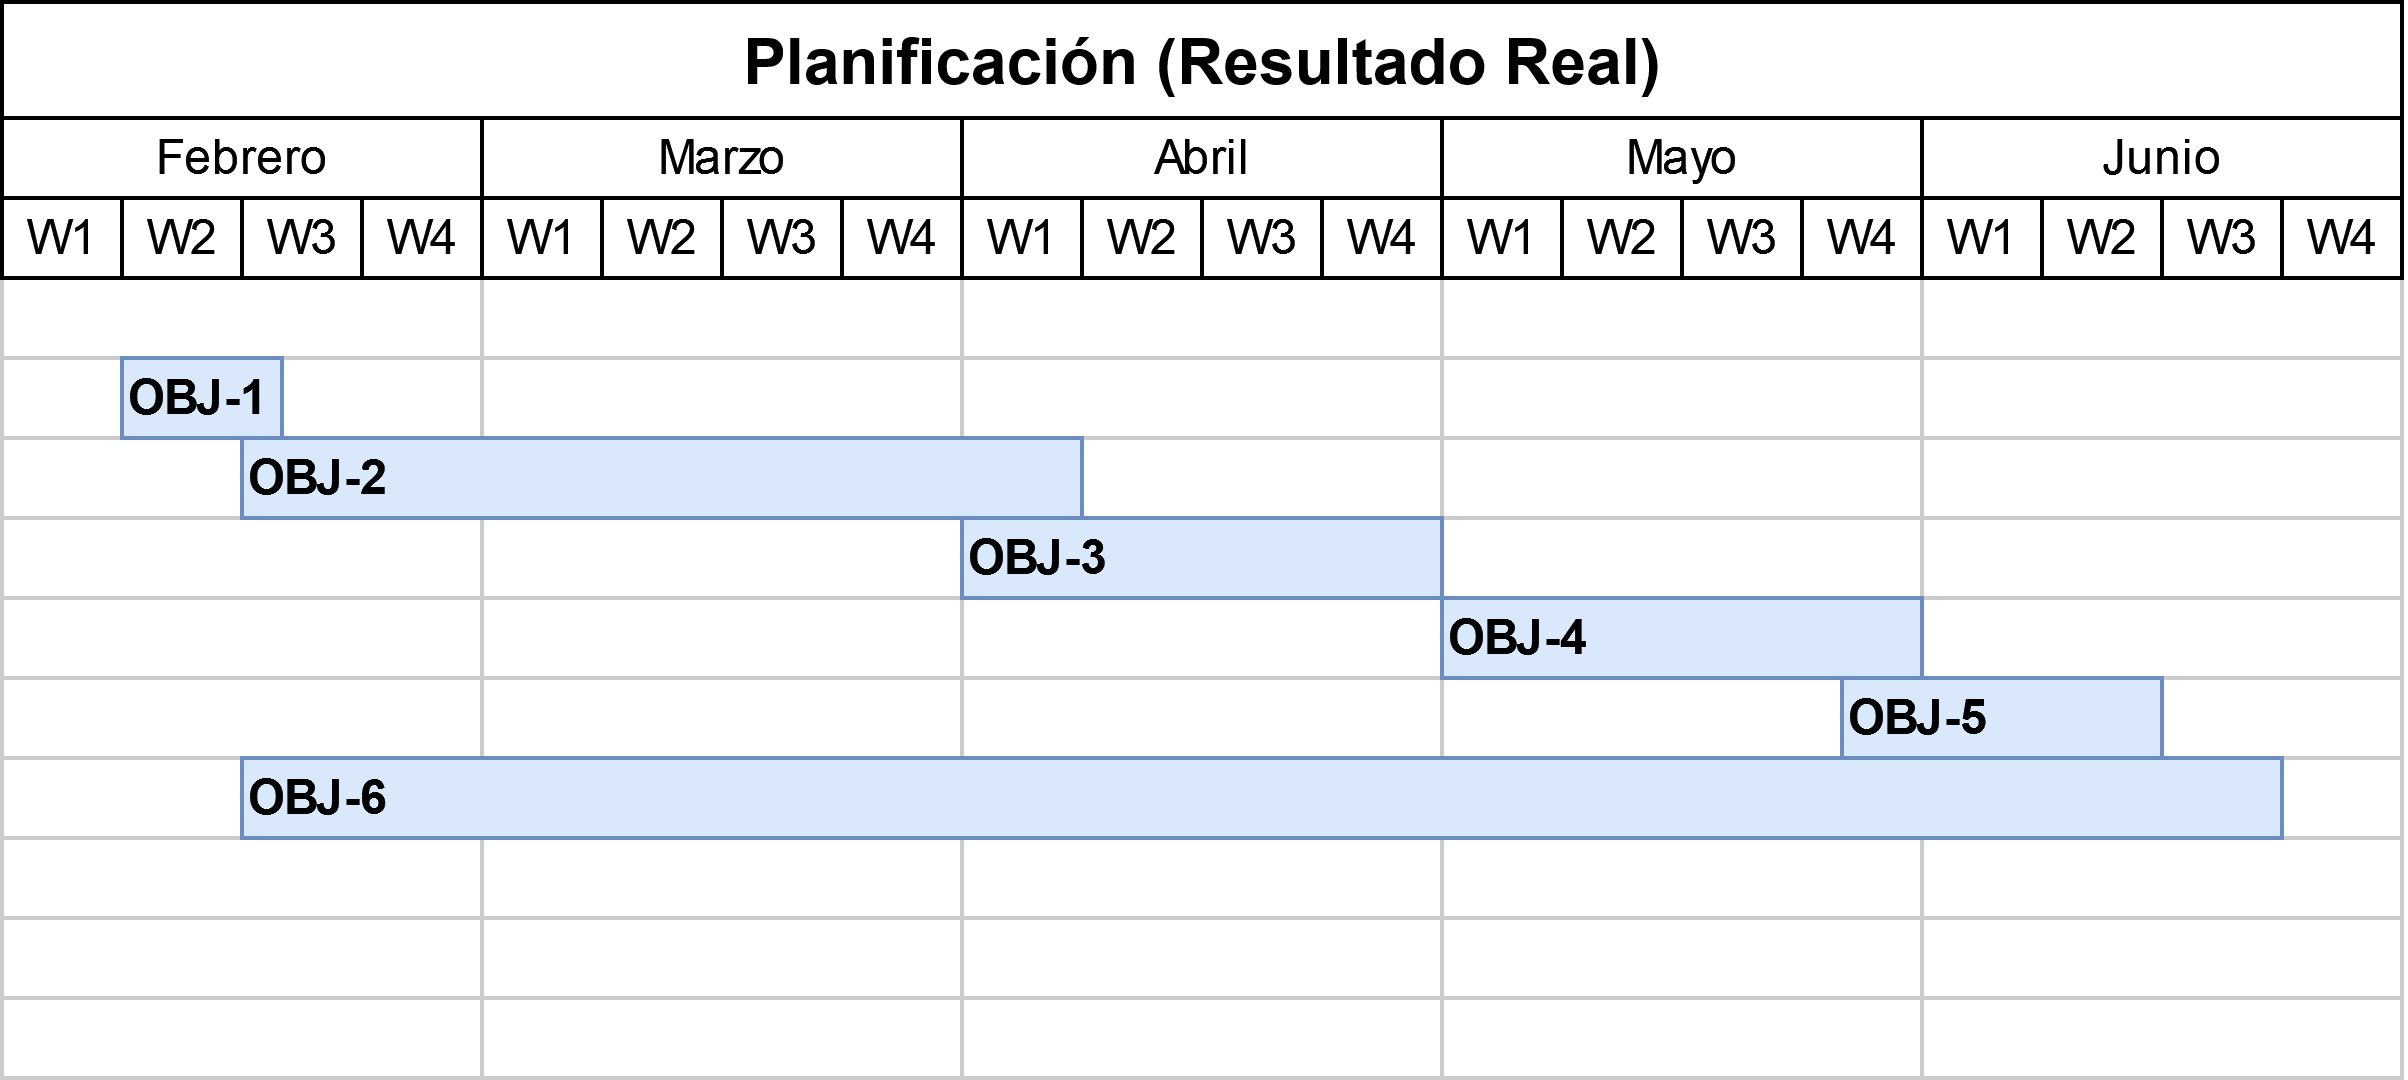
\includegraphics[width=0.99\textwidth]{img/fig/fig5.1-gantt-real.png}
    \caption{Resultados reales de la planificación}
    \label{fig:gantt-real}
\end{figure}

En general, los dos mayores cambios se realizaron en el objetivo 2 y 6 
respecto a la planificación inicial en la \autoref{fig:gantt}.
Se encontraron multitud de problemas durante el objetivo 2 que necesitaron 
mucho más tiempo del planeado, cómo fallos en el firmware de Paparazzi para el Crazyflie. 
Esto provocó un desplazamiento de los objetivos posteriores y se tuvieron que realizar un poco más deprisa.

Por otro lado, el objetivo 6 se decidió realizarse paralelamente al resto de objetivos,
es decir, se realizaban cambios y revisiones casi constantemente, así como se realizaba la memoria en paralelo con lo que se iba desarrollando. 
Esto último permitió que fuese más cómodo escribir la memoria, 
al ir plasmando lo recientemente aprendido sobre esta antes de que se olvidasen detalles en las semanas posteriores. 

%%%%%%%%%%%%%%%%%%%%%%%%%%%%%%%%%%%%%%%%%%%%%%%%%%%%%%%%%%%%%%%%%%%%%%%%%%%%%%%%%%%%%%%%%%%%%%%%%%%%%%%%%%%%%%%%%
%%%%%%%%%%%%%%%%%%%%%%%%%%%%%%%%%%%%%%%%%%%%%%%%%%%%%%%%%%%%%%%%%%%%%%%%%%%%%%%%%%%%%%%%%%%%%%%%%%%%%%%%%%%%%%%%%
%%%%%%%%%%%%%%%%%%%%%%%%%%%%%%%%%%%%%%%%%%%%%%%%%%%%%%%%%%%%%%%%%%%%%%%%%%%%%%%%%%%%%%%%%%%%%%%%%%%%%%%%%%%%%%%%%

\section{Aplicaciones y usos}

Conseguidos los fundamentos de esta tecnología de coordinación, es importante analizar las posibles aplicaciones finales.
Entre ellas, destaca principalmente la experimentación e investigación de la tecnología, 
ya que este trabajo consigue directamente esta aplicación sin mayores modificaciones y adiciones extra.

Además, la base de esta tecnología permite otros usos (por supuesto, con previas modificaciones si fuesen necesarias) 
como pueden ser la vigilancia mediante enjambres de drones, aplicaciones en agricultura, defensa o 
espectáculos de drones independientes del control por \textit{waypoints} fijados por una estación central. 

Es evidente que para terminar de ver las posibles aplicaciones y usos, 
se ha de ver que ha de mejorarse antes, por ello, lo exploraremos en la siguiente subsección.

%%%%%%%%%%%%%%%%%%%%%%%%%%%%%%%%%%%%%%%%%%%%%%%%%%%%%%%%%%%%%%%%%%%%%%%%%%%%%%%%%%%%%%%%%%%%%%%%%%%%%%%%%%%%%%%%%
%%%%%%%%%%%%%%%%%%%%%%%%%%%%%%%%%%%%%%%%%%%%%%%%%%%%%%%%%%%%%%%%%%%%%%%%%%%%%%%%%%%%%%%%%%%%%%%%%%%%%%%%%%%%%%%%%
%%%%%%%%%%%%%%%%%%%%%%%%%%%%%%%%%%%%%%%%%%%%%%%%%%%%%%%%%%%%%%%%%%%%%%%%%%%%%%%%%%%%%%%%%%%%%%%%%%%%%%%%%%%%%%%%%

\section{Trabajos y mejoras futuras}

Si se desease mejorar o continuar sobre la base de este trabajo, las primeras mejoras que se deberían aplicar serían las siguientes:

\begin{itemize}
    \item \textbf{Mejor control en Paparazzi:} al ser el primer objetivo parcialmente no cumplido, es evidente que se necesita mejor control bajo el software de Paparazzi, 
    ya que este es bastamente superado por el software oficial para los Crazyflie.

    \item \textbf{Coordinación real en Paparazzi:} consecuencia de no poder conseguir el correcto control en Paparazzi, es evidente que esto también es necesario corregirlo. 
    Es posible que consiguiendo arreglar el control no se necesite más, pero no es seguro.

    \item \textbf{Implementación para $N$ drones:} si bien el algoritmo se ha diseñado pensando en varios drones, las implementaciones se han simplificado para tan sólo dos drones. 
    Por suerte, esta mejora solo requiere cambios a la hora de introducir los parámetros de desajuste deseado y los calculos respecto a estos.

    \item \textbf{Implementación y uso de otros sistemas de posicionamiento:} 
    como bien se vio en el capítulo 1, existen más sistemas de posicionamiento compatibles con los Crazyflies.
    Estos sistemas podrían dar mayor precisión, evitar acumulación de error e incluso ayudar a la hora de implementar mejor control en Paparazzi. 
\end{itemize}

Por supuesto, esto son las mejoras directas a este TFG, si hablamos de trabajos más grandes a mayor plazo sobre esta tecnología, podemos hablar de lo siguiente:

\begin{itemize}
    \item \textbf{Implementación de GVF paramétrico:} una versión para trayectorias en tres dimensiones de GVF. Más compleja, parcialmente implementada en Paparazzi.

    \item \textbf{Mejoras diversas al software de Paparazzi:} como puede ser mayor facilidad de uso, corregir las simulaciones para el Crazyflie (aunque se pueden usar otros drones), mejorar la documentación, simplificar el software en cuestión de características (son muchas)...

    \item \textbf{Mejora general de los algoritmos:} si bien son buenos, es interesante ver hasta que punto se pueden conseguir algoritmos con mucha mayor precisión, donde el error es mínimo. También se pueden hacer algoritmos más inteligentes, que no solo sigan trayectorias semi-predefinidas.

    \item \textbf{Coordinación descentralizada y distribuida:} aplicar estos conceptos pero sin haber un nodo central, en este caso, el ordenador que controla todo. En otras palabras, coordinar $N$ drones que se comunican entre ellos y deciden que hacer sólos en base a estos algoritmos, sin un PC central que los coordine a todos.

    \item \textbf{Aplicaciones reales:} como puede ser espectáculos de luces basados en GVF, en vez de ser scripts de a que posición debe ir cada dron (como es hoy en día, generalmente).
\end{itemize}

%%%%%%%%%%%%%%%%%%%%%%%%%%%%%%%%%%%%%%%%%%%%%%%%%%%%%%%%%%%%%%%%%%%%%%%%%%%%%%%%%%%%%%%%%%%%%%%%%%%%%%%%%%%%%%%%%
%%%%%%%%%%%%%%%%%%%%%%%%%%%%%%%%%%%%%%%%%%%%%%%%%%%%%%%%%%%%%%%%%%%%%%%%%%%%%%%%%%%%%%%%%%%%%%%%%%%%%%%%%%%%%%%%%
%%%%%%%%%%%%%%%%%%%%%%%%%%%%%%%%%%%%%%%%%%%%%%%%%%%%%%%%%%%%%%%%%%%%%%%%%%%%%%%%%%%%%%%%%%%%%%%%%%%%%%%%%%%%%%%%%

\section{Conclusión}

En conclusión, este trabajo ha conseguido mayoritariamente sus objetivos, planificación y permite diversos usos. 
Se ha demostrado el buen funcionamiento de los algoritmos de estilo GVF y se han probado dos algoritmos de coordinación, uno diseñado en exclusiva para este trabajo.

Los resultados, si bien prometedores, hacen los Crazyflies ideales exclusivamente para la experimentación, investigación y educación 
en el ámbito de control y coordinación de enjambres de drones, debido a las mejoras que aún pueden añadirse, como el mejor control en Paparazzi.

Para conseguir más aplicaciones y usos, es recomendable la adición de otros componentes a este trabajo, 
como pueden ser cámaras (para vigilancia) o LEDs (para espectáculos de luces), 
así como el desarrollo extra en mejorar tanto el control como la coordinación e 
incluso avances de hardware que escapan al ámbito de este trabajo.